
\subsubsection{Thorの初期化}
\begin{figure}[htbp]\begin{center}
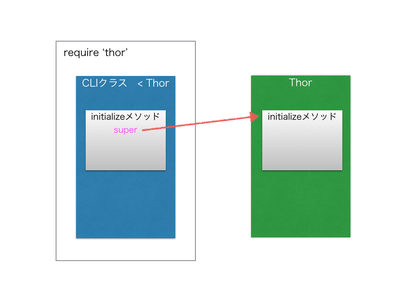
\includegraphics[width=6cm,bb=0 0 442 500]{../figs/./hikiutils_yamane_09_copy.003.jpg}
\caption{}
\label{default}\end{center}\end{figure}
\begin{itemize}
\item Thorのinitializeでのコード
\end{itemize}
\begin{enumerate}
\item Hikithor::CLI.start(ARGV)が呼ばれる
\item initializeメソッドが呼ばれる
\item これではThorのinitializeメソッドが呼ばれない
\item superを書くことでThorのinitializeメソッドが呼ばれる
\end{enumerate}
optparseではrequireでoptparseを呼びoptparseのinitializeを定義する必要はないが,Thorはinitializeを定義する必要がある.
Thorの定義方法はrequireでThorを呼びCLIクラスで継承し,initializeメソッドにsuperを書くことでThorのinitializeが呼ばれる.
initializeメソッド内ではThorの初期設定がされていないため,スーパークラスのメソッドを読み出してくれるsuperを書き加えることで図のようにinitializeメソッド内でThorのinitilalizeメソッドが
呼ばれ定義される.

\paragraph{コード}\begin{lstlisting}[style=customRuby]
# -*- coding: utf-8 -*-                                                         
require 'thor'
require 'kconv'
require 'hikidoc'
require 'erb'
require "hikiutils/version"
require "hikiutils/tmarshal"
require "hikiutils/infodb"
require 'systemu'
require 'fileutils'
require 'yaml'
require 'pp'

module Hikithor

  DATA_FILE=File.join(ENV['HOME'],'.hikirc')
  attr_accessor :src, :target, :editor_command, :browser, :data_name, :l_dir

  class CLI < Thor
   def initialize(*args)
      super
      @data_name=['nick_name','local_dir','local_uri','global_dir','global_uri']
      data_path = File.join(ENV['HOME'], '.hikirc')
      DataFiles.prepare(data_path)

      file = File.open(DATA_FILE,'r')
      @src = YAML.load(file.read)
      file.close
      @target = @src[:target]
      @l_dir=@src[:srcs][@target][:local_dir]
      browser = @src[:browser]
      @browser = (browser==nil) ? 'firefox' : browser
      p editor_command = @src[:editor_command]
      @editor_command = (editor_command==nil) ? 'open -a mi' : editor_command
   end
\end{lstlisting}
\subsubsection{コマンド表示と処理}
\paragraph{Thor}
\begin{figure}[htbp]\begin{center}
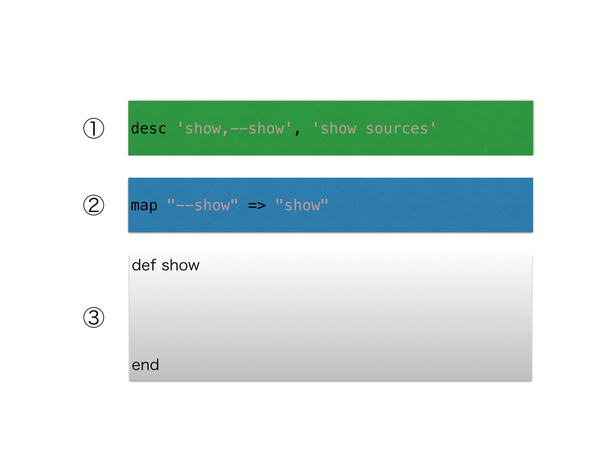
\includegraphics[width=6cm,bb=0 0 442 500]{../figs/./hikiutils_yamane_09_copy.004.jpg}
\caption{}
\label{default}\end{center}\end{figure}
\begin{enumerate}
\item コマンド名,コマンドの説明を一覧に表示させる
\item パブリックメソッドのコマンドを別のコマンド名でも実行できるようにする
\item コマンドの命令の実行コード
\end{enumerate}
Thorではdescで一覧を表示させるコマンド名,コマンドの説明を登録する.しかし,ここで記述したコマンドは一覧で表示させるものであり,実行されることはないので実際のコマンドと対応させる必要がある.
Thorでは処理実行を行うメソッドがコマンドとなる.しかし,それではコマンド名は1つしか使うことができない.
ここで用いるものがmapである.
\begin{quote}\begin{verbatim}
map A => B
\end{verbatim}\end{quote}
mapとはBでしか読めないものをAでも読めるようにしてくれるものである.
よって,これを使うことで別のコマンドも指定することができる.

\paragraph{optparse}
\begin{figure}[htbp]\begin{center}
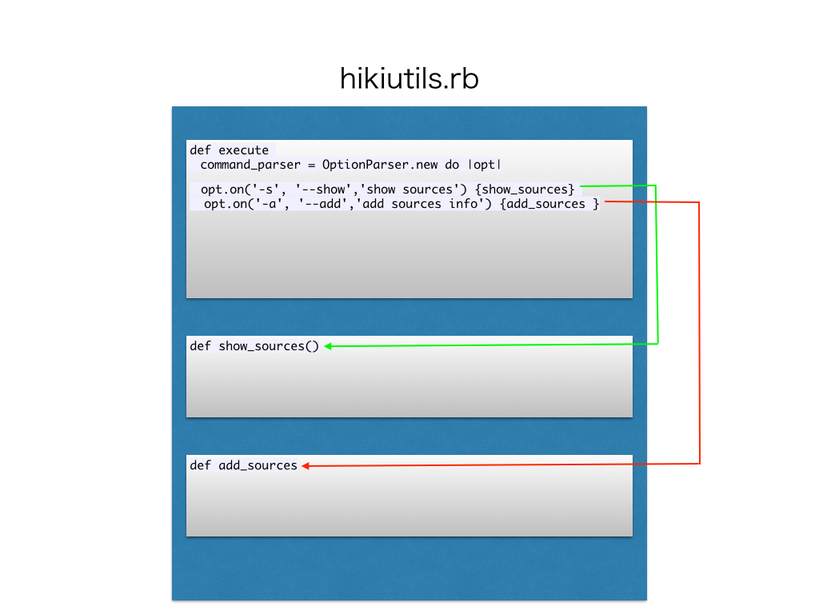
\includegraphics[width=6cm,bb=0 0 442 500]{../figs/./hikiutils_yamane_09_copy.005.jpg}
\caption{}
\label{default}\end{center}\end{figure}
\begin{enumerate}
\item OptionParserオブジェクトoptを生成
\item optにコマンドを登録
\item 入力されたコマンドの処理のメソッドへ移動
\end{enumerate}
optparseではOptionParserオブジェクトoptの生成を行い,コマンドをoptに登録することでコマンドを作成することができる.しかし,これはコマンドを登録しているだけで
コマンドの一覧ではこれを表示することができるが,コマンドの実行を行うためには実行を行うためのメソッドを作成する必要がある.optparseでのコマンドの実行はoptで登録された
コマンドが入力されることでそれぞれのコマンドの処理を行うメソッドに移動し処理を行う.しかし,このコマンド登録はハイフンを付けたコマンドしか登録ができず,ハイフンなしのコマンド登録は
また別の手段でやらなくてはいけない.
以上より,Thorではコマンドの指定と処理にはdesc,map,処理メソッドだけで済むが,optparseではコマンドを登録するためのメソッドと処理メソッドが必要になってくる.
また,コマンドはThorでは処理メソッドがコマンド名になるが,optparseではコマンドを登録するための処理も必要となってくる.

\paragraph{コード}
\begin{itemize}
\item Thor
\end{itemize}\begin{lstlisting}[style=customRuby]
    desc 'show,--show', 'show sources'
    map "--show" => "show"
    def show
      printf("target_no:%i\n",@src[:target])
      printf("editor_command:%s\n",@src[:editor_command])
      @i_size,@n_size,@l_size,@g_size=3,5,30,15 #i,g_size are fixed             
      n_l,l_l=0,0
      @src[:srcs].each_with_index{|src,i|
        n_l =(n_l= src[:nick_name].length)>@n_size? n_l:@n_size
        l_l =(l_l= src[:local_dir].length)>@l_size? l_l:@l_size
      }
      @n_size,@l_size=n_l,l_l
      command = Command.new
      header = command.display_format('id','name','local directory','global uri',@i_size,@n_size,@l_size,@g_size)

      puts header
      puts '-' * header.size

      @src[:srcs].each_with_index{|src,i|
        target = i==@src[:target] ? '*':' '
        id = target+i.to_s
        name=src[:nick_name]
        local=src[:local_dir]
        global=src[:global_uri]
        puts command.display_format(id,name,local,global,@i_size,@n_size,@l_size,@g_size)
      }
    end
\end{lstlisting}
\begin{itemize}
\item optparse
\end{itemize}\begin{lstlisting}[style=customRuby]
    def execute
      @argv << '--help' if @argv.size==0
      command_parser = OptionParser.new do |opt|
        opt.on('-v', '--version','show program Version.') { |v|
          opt.version = HikiUtils::VERSION
          puts opt.ver
        }
        opt.on('-s', '--show','show sources') {show_sources}
        opt.on('-a', '--add','add sources info') {add_sources }
        opt.on('-t', '--target VAL','set target id') {|val| set_target(val)}
        opt.on('-e', '--edit FILE','open file') {|file| edit_file(file) }
        opt.on('-l', '--list [FILE]','list files') {|file| list_files(file)}
        opt.on('-u', '--update FILE','update file') {|file| update_file(file) }
        opt.on('-r', '--rsync','rsync files') {rsync_files}
        opt.on('--database FILE','read database file') {|file| db_file(file)}
        opt.on('--display FILE','display converted hikifile') {|file| display(file)}
        opt.on('-c', '--checkdb','check database file') {check_db}
        opt.on('--remove FILE','remove file') {|file| remove_file(file)}
        opt.on('--move FILES','move file1,file2',Array) {|files| move_file(files)}
        opt.on('--euc FILE','translate file to euc') {|file| euc_file(file)}
        opt.on('--initialize','initialize source directory') {dir_init() }
      end
      begin
        command_parser.parse!(@argv)
      rescue=> eval
        p eval
      end
      dump_sources
      exit
    end    
    
    def show_sources()
      printf("target_no:%i\n",@src[:target])
      printf("editor_command:%s\n",@src[:editor_command])
      check_display_size()
      header = display_format('id','name','local directory','global uri')

      puts header
      puts '-' * header.size

      @src[:srcs].each_with_index{|src,i|
        target = i==@src[:target] ? '*':' '
        id = target+i.to_s
        name=src[:nick_name]
        local=src[:local_dir]
        global=src[:global_uri]
        puts display_format(id,name,local,global)
      }
    end

    def add_sources
      cont = {}
      @data_name.each{|name|
        printf("%s ? ", name)
        tmp = gets.chomp
        cont[name.to_sym] = tmp
      }
      @src[:srcs] << cont
      show_sources
    end
\end{lstlisting}
\subsubsection{CLIの実行}
\paragraph{Thor}
\begin{figure}[htbp]\begin{center}
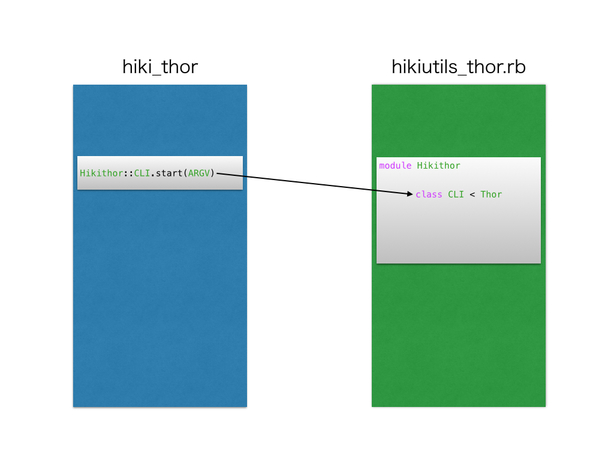
\includegraphics[width=6cm,bb=0 0 442 500]{../figs/./hikiutils_yamane_09_copy.006.jpg}
\caption{}
\label{default}\end{center}\end{figure}
\begin{itemize}
\item 実行手順
\end{itemize}
\begin{enumerate}
\item hiki\_thorのHikithor::CLI.start(ARGV)でhikiutils\_thor.rbのCLIクラスを呼ぶ
\item hikiutils\_thor.rbのCLIクラスのメソッドを順に実行していく
\end{enumerate}
Thorではstart(ARGV)を呼び出すことでCLIを開始する.Hikithor::CLI.start(ARGV)を実行されることによりrequireで呼ばれているhikiutils\_thor.rbのCLIコマンドを順に実行する.
そして,入力されたコマンドと一致するメソッドを探し,そのコマンドの処理が実行される.

\paragraph{optparse}
\begin{figure}[htbp]\begin{center}
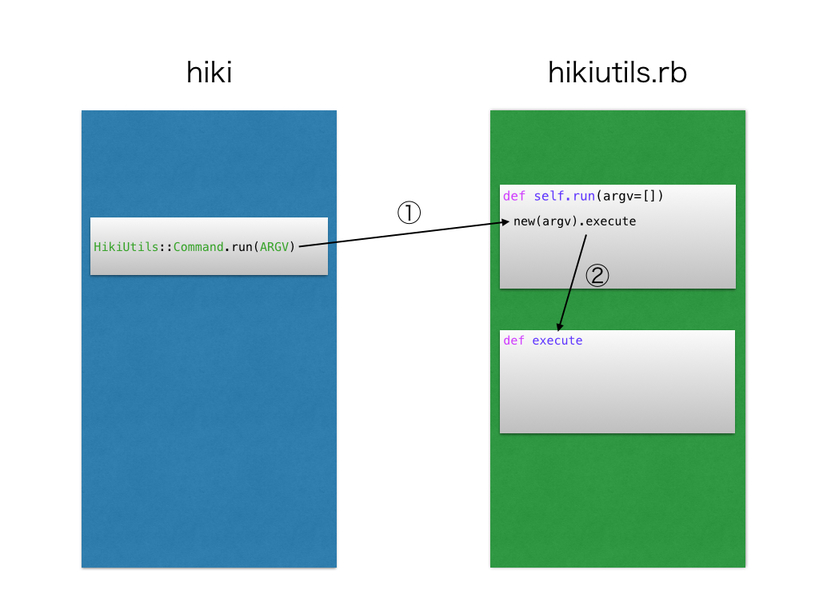
\includegraphics[width=6cm,bb=0 0 442 500]{../figs/./hikiutils_yamane_09_copy.007.jpg}
\caption{}
\label{default}\end{center}\end{figure}
\begin{itemize}
\item 実行手順
\end{itemize}
\begin{enumerate}
\item HikiのHikiUtils::Command.run(ARGV)でhikiutils.rbのrunメソッドを呼ぶ
\item new(argv).executeでexecuteメソッドが実行される
\end{enumerate}
一方,optparseではHikiutils::Command.run(ARGV)を実行される.requireで呼び出されたhikiutils.rbでrunメソッドが実行される.
そこでコマンドを登録しているexecuteメソッドへ移動し入力したコマンドと対応させる.そして,対応したコマンドの処理が行われるメソッドに移動することで実行される.
このようにoptparseでは実行を行うためのメソッドが必要であるが,Thorではクラスのメソッドを順に実行していくため
runメソッドとexecuteメソッドは必要ない.また,optparseでの実行手順はメソッドの移動回数が多く複雑であるが,Thorは単純で分かりやすいものとなっている.

\paragraph{コード}
\begin{itemize}
\item Thor
\end{itemize}\begin{lstlisting}[style=customRuby]
#!/usr/bin/env ruby                                                             

require "hikiutils_thor"

Hikithor::CLI.start(ARGV)
\end{lstlisting}\begin{lstlisting}[style=customRuby]
# -*- coding: utf-8 -*-                                                         
require 'thor'
require 'kconv'
require 'hikidoc'
require 'erb'
require "hikiutils/version"
require "hikiutils/tmarshal"
require "hikiutils/infodb"
require 'systemu'
require 'fileutils'
require 'yaml'
require 'pp'

module Hikithor

  DATA_FILE=File.join(ENV['HOME'],'.hikirc')
  attr_accessor :src, :target, :editor_command, :browser, :data_name, :l_dir

  class CLI < Thor
   def initialize(*args)
      super
      @data_name=['nick_name','local_dir','local_uri','global_dir','global_uri']
      data_path = File.join(ENV['HOME'], '.hikirc')
      DataFiles.prepare(data_path)

      file = File.open(DATA_FILE,'r')
      @src = YAML.load(file.read)
      file.close
      @target = @src[:target]
      @l_dir=@src[:srcs][@target][:local_dir]
      browser = @src[:browser]
      @browser = (browser==nil) ? 'firefox' : browser

\end{lstlisting}
\begin{itemize}
\item optparse
\end{itemize}\begin{lstlisting}[style=customRuby]
#!/usr/bin/env ruby                                                             

require "hikiutils"

HikiUtils::Command.run(ARGV)
\end{lstlisting}\begin{lstlisting}[style=customRuby]
    def self.run(argv=[])
      print "hikiutils: provide utilities for helping hiki editing.\n"
      new(argv).execute
    end

    def execute
      @argv << '--help' if @argv.size==0
      command_parser = OptionParser.new do |opt|
        opt.on('-v', '--version','show program Version.') { |v|
          opt.version = HikiUtils::VERSION
          puts opt.ver
        }
        opt.on('-s', '--show','show sources') {show_sources}
        opt.on('-a', '--add','add sources info') {add_sources }
        opt.on('-t', '--target VAL','set target id') {|val| set_target(val) }
        opt.on('-e', '--edit FILE','open file') {|file| edit_file(file) }
        opt.on('-l', '--list [FILE]','list files') {|file| list_files(file) }
        opt.on('-u', '--update FILE','update file') {|file| update_file(file) }
        opt.on('-r', '--rsync','rsync files') {rsync_files}
        opt.on('--database FILE','read database file') {|file| db_file(file)}
        opt.on('--display FILE','display converted hikifile') {|file| display(f\
ile)}
        opt.on('-c', '--checkdb','check database file') {check_db}
        opt.on('--remove FILE','remove file') {|file| remove_file(file)}
        opt.on('--move FILES','move file1,file2',Array) {|files| move_file(file\
s)}
        opt.on('--euc FILE','translate file to euc') {|file| euc_file(file) }
        opt.on('--initialize','initialize source directory') {dir_init() }
      end
      begin
        command_parser.parse!(@argv)
      rescue=> eval
        p eval
      end
      dump_sources
      exit
    end  
\end{lstlisting}
コードからもThorのほうが短くなっていることが分かる.
よって,Thorとoptparseでのコードの違いは以上の部分になるが全体的にもThorのほうがコードが短くなり,
コマンドの定義も簡単に行うことができる.また,実行手順も分かりやすくコードが読みやすいため書き換えもすぐ行うことが
できるので,より直感的なコマンドを実装することも可能となった.

